
%%%%%%%%%%%%%%%%%%%%%%%%%%%%%%%%%%%%%%%%%%%%%%%%%%%%%%%%%%%%%%%%%%%%%%%%%%%%%%%%%%%%%%%
%%%%%%%%%%%%%%%%%%%%%%%%%%%%%%%%%%%%%%%%%%%%%%%%%%%%%%%%%%%%%%%%%%%%%%%%%%%%%%%%%%%%%%%
% 
% This top part of the document is called the 'preamble'.  Modify it with caution!
%
% The real document starts below where it says 'The main document starts here'.

\documentclass[12pt]{article}

\usepackage{amssymb,amsmath,amsthm}
\usepackage[top=1in, bottom=1in, left=1.25in, right=1.25in]{geometry}
\usepackage{fancyhdr}
\usepackage{enumerate}
\usepackage{listings}
\usepackage{graphicx}
\usepackage{float}

\usepackage{mwe}
\usepackage{caption}
\usepackage{subcaption}
% Comment the following line to use TeX's default font of Computer Modern.
\usepackage{times,txfonts}



\makeatletter
\renewcommand*\env@matrix[1][*\c@MaxMatrixCols c]{%
  \hskip -\arraycolsep
  \let\@ifnextchar\new@ifnextchar
  \array{#1}}
\makeatother

\newtheoremstyle{homework}% name of the style to be used
  {18pt}% measure of space to leave above the theorem. E.g.: 3pt
  {12pt}% measure of space to leave below the theorem. E.g.: 3pt
  {}% name of font to use in the body of the theorem
  {}% measure of space to indent
  {\bfseries}% name of head font
  {:}% punctuation between head and body
  {2ex}% space after theorem head; " " = normal interword space
  {}% Manually specify head
\theoremstyle{homework} 

% Set up an Exercise environment and a Solution label.
\newtheorem*{exercisecore}{Exercise \@currentlabel}
\newenvironment{exercise}[1]
{\def\@currentlabel{#1}\exercisecore}
{\endexercisecore}

\newcommand{\localhead}[1]{\par\smallskip\noindent\textbf{#1}\nobreak\\}%
\newcommand\solution{\localhead{Solution:}}

%%%%%%%%%%%%%%%%%%%%%%%%%%%%%%%%%%%%%%%%%%%%%%%%%%%%%%%%%%%%%%%%%%%%%%%%
%
% Stuff for getting the name/document date/title across the header
\makeatletter
\RequirePackage{fancyhdr}
\pagestyle{fancy}
\fancyfoot[C]{\ifnum \value{page} > 1\relax\thepage\fi}
\fancyhead[L]{\ifx\@doclabel\@empty\else\@doclabel\fi}
\fancyhead[C]{\ifx\@docdate\@empty\else\@docdate\fi}
\fancyhead[R]{\ifx\@docauthor\@empty\else\@docauthor\fi}
\headheight 15pt

\def\doclabel#1{\gdef\@doclabel{#1}}
\doclabel{Use {\tt\textbackslash doclabel\{MY LABEL\}}.}
\def\docdate#1{\gdef\@docdate{#1}}
\docdate{Use {\tt\textbackslash docdate\{MY DATE\}}.}
\def\docauthor#1{\gdef\@docauthor{#1}}
\docauthor{Use {\tt\textbackslash docauthor\{MY NAME\}}.}
\makeatother

% Shortcuts for blackboard bold number sets (reals, integers, etc.)
\newcommand{\Reals}{\ensuremath{\mathbb R}}
\newcommand{\Nats}{\ensuremath{\mathbb N}}
\newcommand{\Ints}{\ensuremath{\mathbb Z}}
\newcommand{\Rats}{\ensuremath{\mathbb Q}}
\newcommand{\Cplx}{\ensuremath{\mathbb C}}
%% Some equivalents that some people may prefer.
\let\RR\Reals
\let\NN\Nats
\let\II\Ints
\let\CC\Cplx
%%%%%%%%%%%%%%%%%%%%%%%%%%%%%%%%%%%%%%%%%%%%%%%%%%%%%%%%%%%%%%%%%%%%%%%%%%%%%%%%%%%%%%%
%%%%%%%%%%%%%%%%%%%%%%%%%%%%%%%%%%%%%%%%%%%%%%%%%%%%%%%%%%%%%%%%%%%%%%%%%%%%%%%%%%%%%%%
% 
% The main document start here.

% The following commands set up the material that appears in the header.




%  \textbf{Code:}
%  \begin{center}
%  \lstinputlisting[basicstyle = \footnotesize]{}
%  \end{center}
%  
%  \begin{footnotesize}
%  \begin{verbatim}
%    
%  \end{verbatim}
%  \end{footnotesize}
%  
%  
%  \begin{figure}[H]
%    \begin{center}
%      \caption{}
%    \includegraphics[width = \textwidth]{}
%    \end{center}
%  \end{figure}




\doclabel{Stat 461: Homework 7}
\docauthor{Stefano Fochesatto}
\docdate{\today}

\begin{document}
\begin{exercise}{1} Read the data in the appendix into R. You will examine the data in 3d:
  \begin{footnotesize}
  \begin{verbatim}
    library(car)
    library(car)
    scatter3d(x1~x2+x3, data=dat, neg.res.col="white",
    pos.res.col="white", surface.alpha=0.0)
  \end{verbatim}
  \end{footnotesize}
  \begin{enumerate}
    \item[a.] Use kmeans to determine the optimal number of clusters, and then plot the 3d plot.\\
    \solution The kmeans algorithm simply finds the optimal partition of the data which reduces the intra-class variance (sum of squared distances from cluster 
    centroids). With that in mind determining an optimal number of clusters is subjective, however we can make an informed decision on how many clusters we should use 
    by examining the ratio between the sum of squares between clusters and the sum of squares total (like $r^2$). The greater this ratio, the more of the variance is explained by our clustering.
    Simulating kmeans for 1 to 10 clusters and computing the $r^2$ we get the following, 
      \begin{figure}[H]
        \begin{center}
          \caption{Plot of $r^2$ up to 10 Clusters.}
        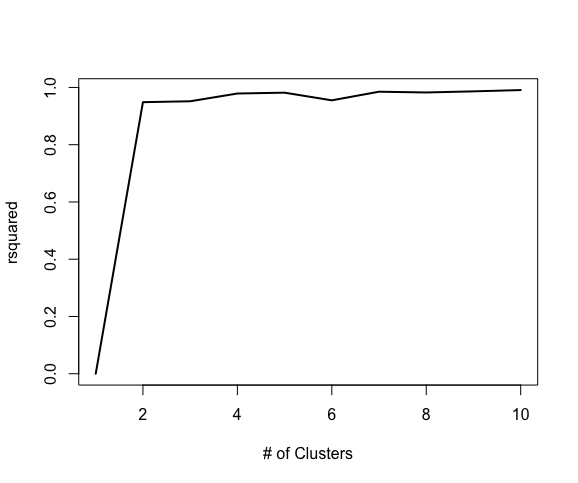
\includegraphics[width = .65\textwidth]{Rplot01.png}
        \end{center}
      \end{figure}
      Clearly we can see that after 2 clusters we are seeing marginal returns on the amount of variance explained. 
      Comparing the 2 clustering and the data, it seems as though 2 clusters is satisfactory, and likely the true signal behind whatever system 
      generated the data. 
        \begin{figure}[H]
          \begin{center}
            \caption{3D Data Plot}
          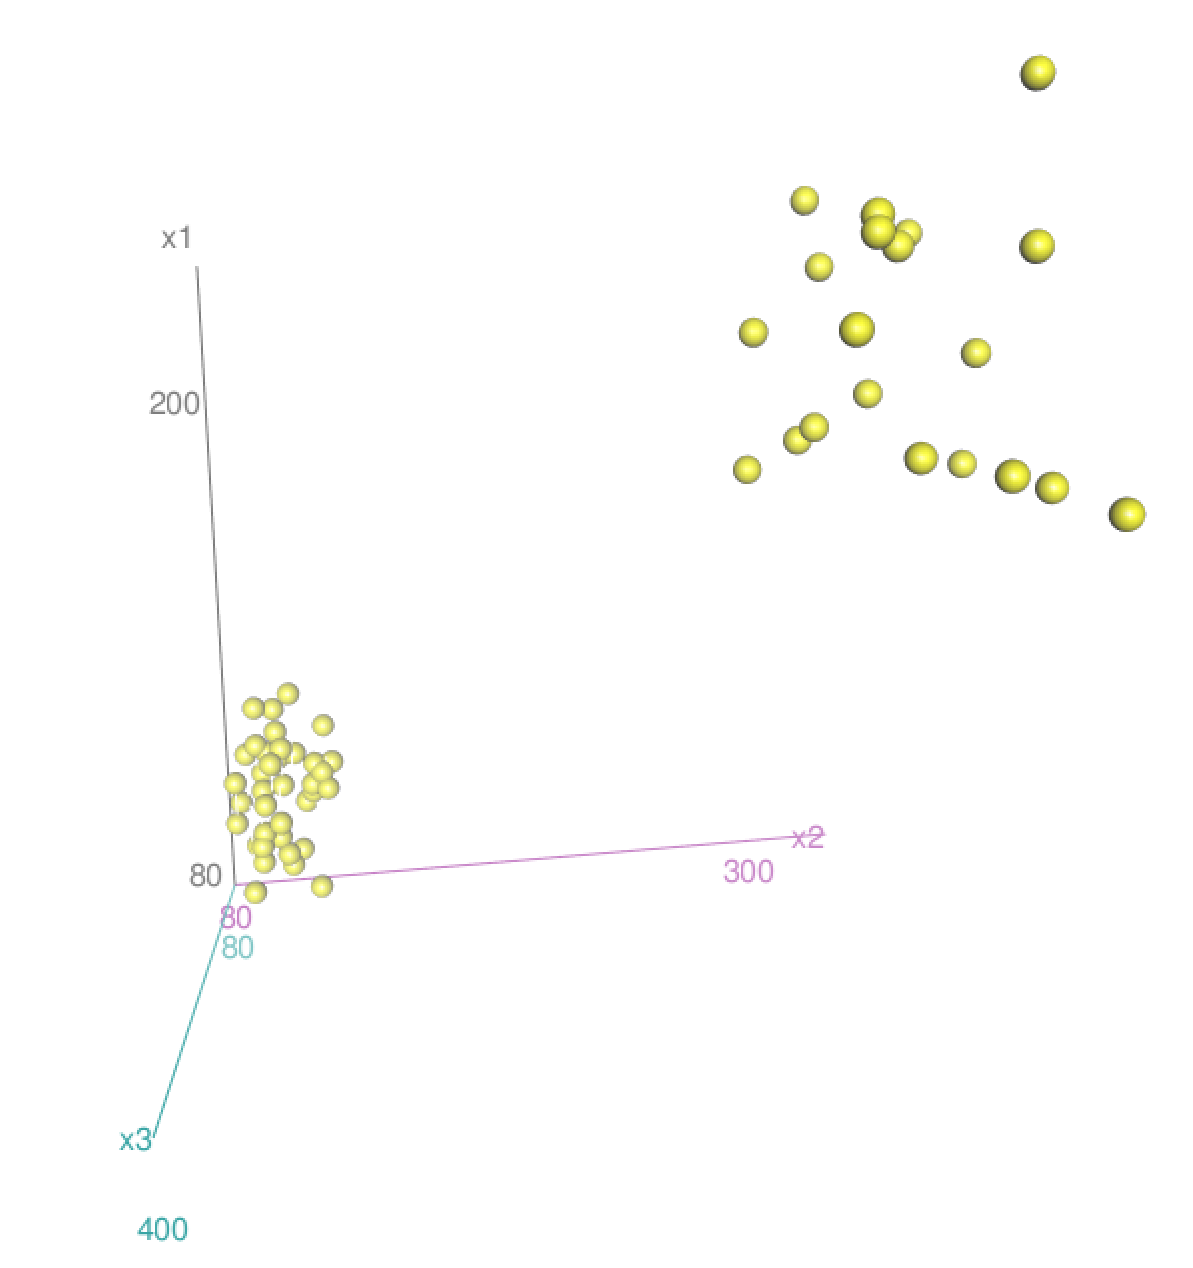
\includegraphics[width = .80\textwidth]{Dat3d.png}
          \end{center}
        \end{figure}
        \begin{figure}[H]
          \begin{center}
            \caption{3D Data Plot With 2 Clusters}
          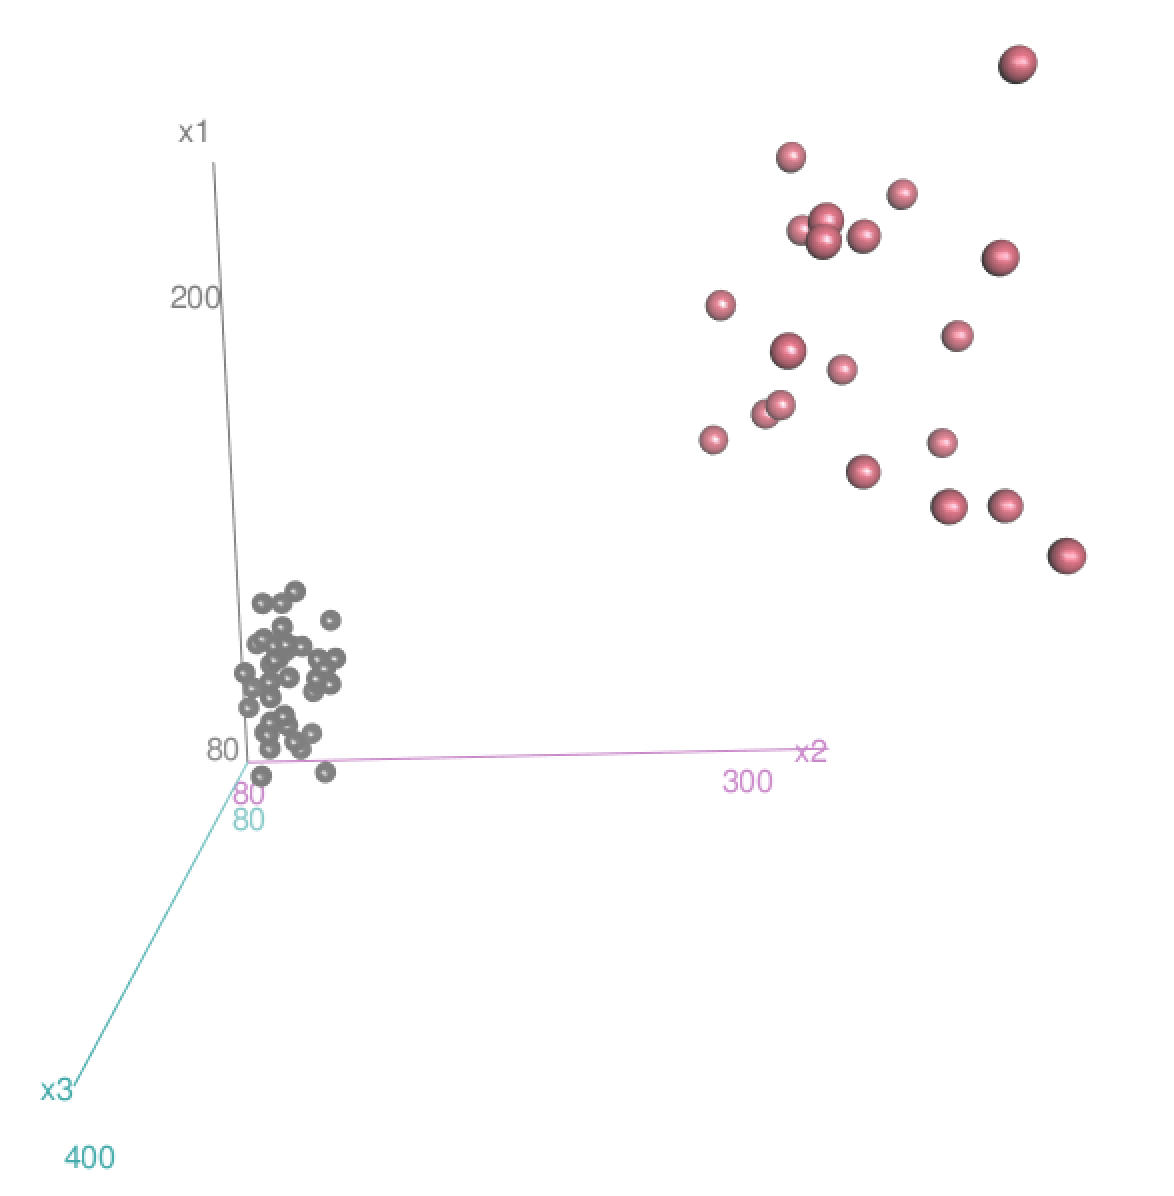
\includegraphics[width = .80\textwidth]{Dat3DClustered.png}
          \end{center}
        \end{figure}
        \vspace{.15in}



      \item[b.] Now use a hierarchical method. Try both complete and single linkage. Do you get the same clustering in the same order for both linkages?\\
      \solution Using an agglomerative hierarchical method with the hclust() function we got the following dendrograms for the given data, using both linkages and euclidean distances,
      \begin{figure}[H]
        \begin{center}
          \caption{Single Linkage}
        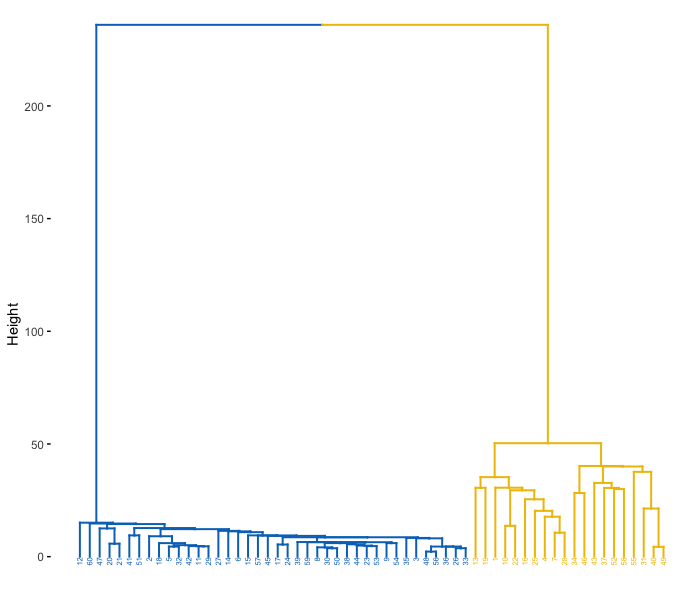
\includegraphics[width = .70\textwidth]{Rplot.png}
        \end{center}
      \end{figure}
      \begin{figure}[H]
        \begin{center}
          \caption{Complete Linkage}
        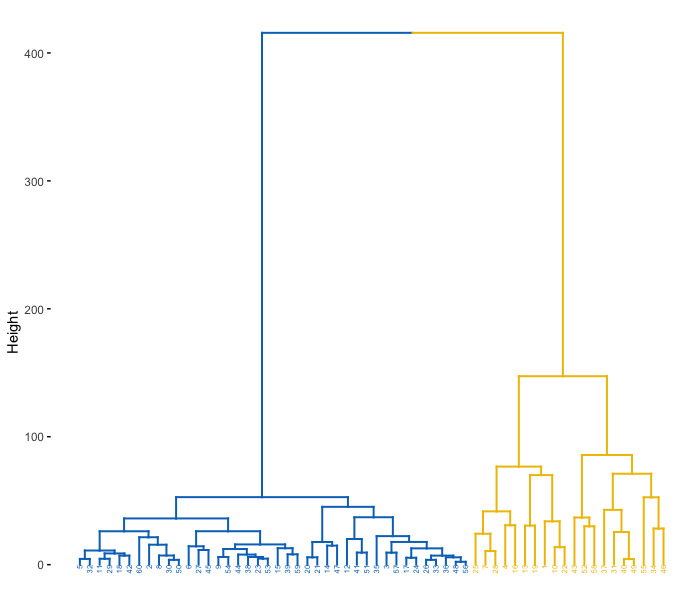
\includegraphics[width = .70\textwidth]{Rplot02.png}
        \end{center}
      \end{figure}
      The following figure shows that each clustering method resulted in the same clusters, however using the order call on the dendrogram object we can see that the order is not the same, 
      \begin{figure}[H]
        \begin{center}
          \caption{Checking Clusters}
        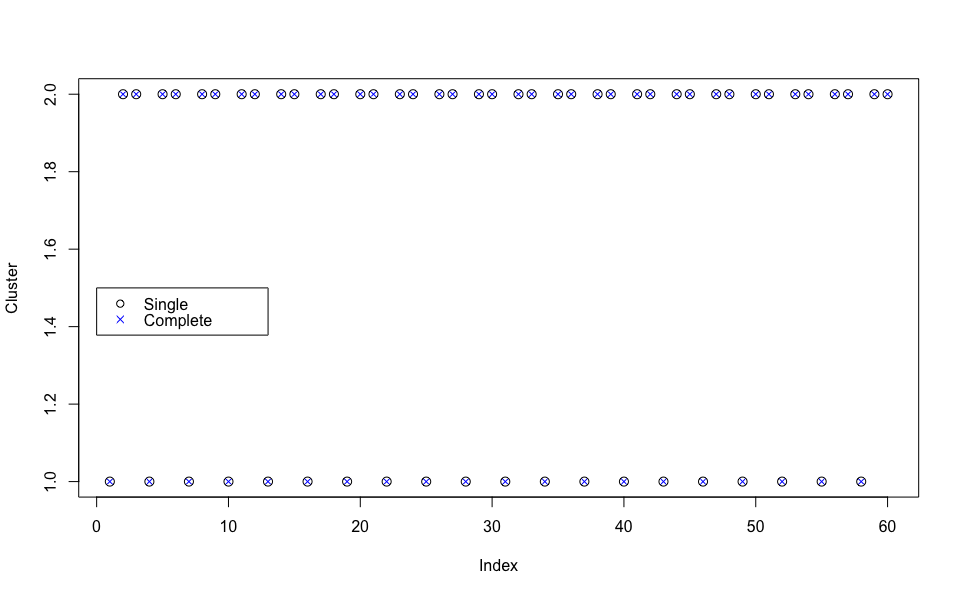
\includegraphics[width = \textwidth]{Rplot03.png}
        \end{center}
      \end{figure}

        \textbf{Code:}
        \begin{center}
        \lstinputlisting[basicstyle = \footnotesize]{r2.txt}
        \end{center}
        \vspace{.15in}



        \item[c.] What is complete linkage? What is single linkage?\\
        \solution Linkage describes how we measure distance between clusters (and clusters and single observations). Suppose $A$ and $B$ are clusters such that 
        $x \in A$ and $y \in B$ then under single linkage we get the following, 
        \begin{equation*}
          d(A,B) = min(x, y).
        \end{equation*}
        Under complete complete linkage we get the following, 
        \begin{equation*}
          d(A,B) = max(x, y).
        \end{equation*}

  \end{enumerate}

\end{exercise}
\vspace{.5in}

\begin{exercise}{2}
  \begin{enumerate}
    \item[a.] Import the Woody Species data set.\\ 
    \solution 
    \textbf{Code:}
    \begin{center}
    \lstinputlisting[basicstyle = \footnotesize]{r3.txt}
    \end{center}
    \vspace{.15in}
    
    \item[b.] Now use kmeans to determine a 'reasonable' number of clusters. You should justify your choice of cluster numbers.\\
    \solution Generating the $r^2$ plot similarly to the first problem we get the following plots, 
    \begin{figure}[H]
      \begin{center}
        \caption{Plot of $r^2$ up to 10 Clusters.}
      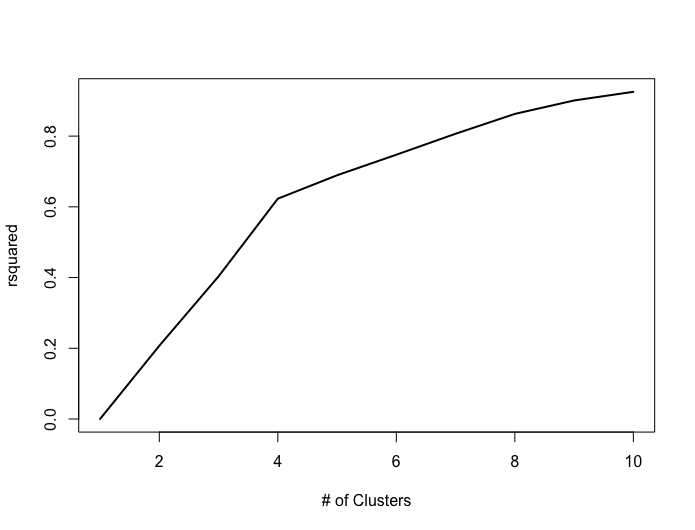
\includegraphics[width = .70\textwidth]{Rplot04.png}
      \end{center}
    \end{figure}
    \begin{figure}[H]
      \begin{center}
        \caption{Proportion of $r^2$ for Each Cluster.(Scree-ish plot)}
      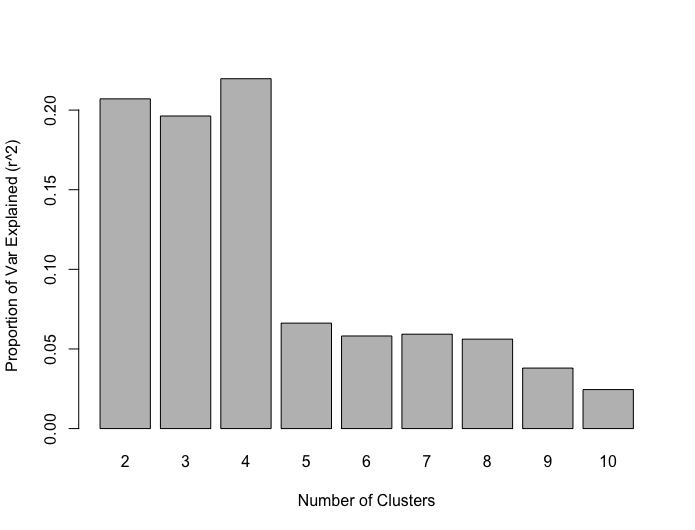
\includegraphics[width = .70\textwidth]{Rplot05.png}
      \end{center}
    \end{figure}
    From here we can see that adding the fifth cluster contributes, marginally to the proportion of variance explained, and therefore I would explore clustering into 4
    or less groups. \\
    \textbf{Code:}
    \begin{center}
    \lstinputlisting[basicstyle = \footnotesize]{r4.txt}
    \end{center}
    \vspace{.15in}


    \item[c.] Briefly, how does kmeans() work?\\
    \solution The kmeans algorithm begins by randomly assigning the data to $n$(hyperparameter) different clusters. Then the centroid of each cluster is computed. 
    The data are reassigned to the same cluster as the nearest centroid. New centroids are computed and the data is reassigned again recursively. Eventually this algorithm 
    converges, and sometimes it shows sensitivity to initial conditions which is why kmeans() runs several randomized instances of this algorithm.
  \vspace{.15in}


  \item[d.] Now cluster the data using any hierarchical clustering method you wish. Don't forget to think about a reasonable distance measure. Do you get similar clusters to when you used kmeans?\\
  \solution Note that the data are stated to be plant densities from each 10 $m^2$ plot. With this mind I think an average linkage and normal
  euclidean distance might be the most appropriate, since are data are already an average in a sense, as opposed to actual plant counts. Generating the dendrogram we get the following, 
  
  \begin{figure}[H]
    \begin{center}
      \caption{Dendrogram for Woody Species Data from hclust() and 'average' Linkage}
    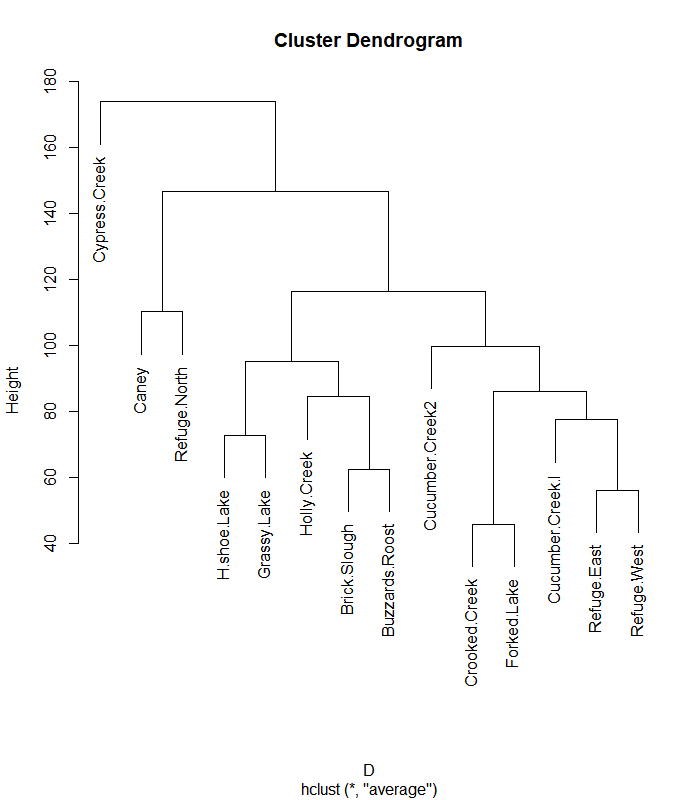
\includegraphics[width = .70\textwidth]{Rplot06.png}
    \end{center}
  \end{figure}
  
  \begin{figure}[H]
    \begin{center}
      \caption{Cut with 3 Clusters (what was done in the paper.)}
    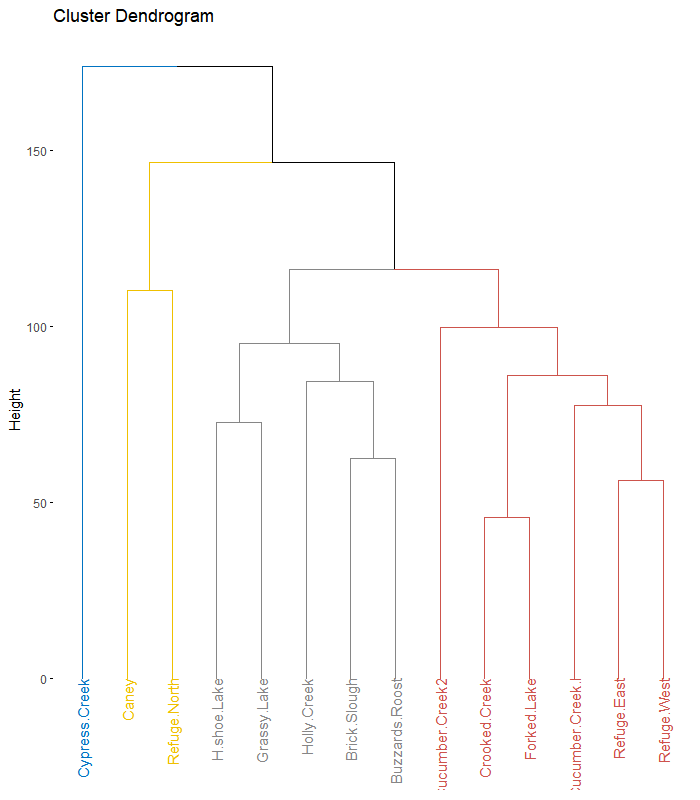
\includegraphics[width = .70\textwidth]{Rplot07.png}
    \end{center}
  \end{figure}

    \begin{figure}[H]
      \begin{center}
        \caption{Cut with 4 Clusters}
      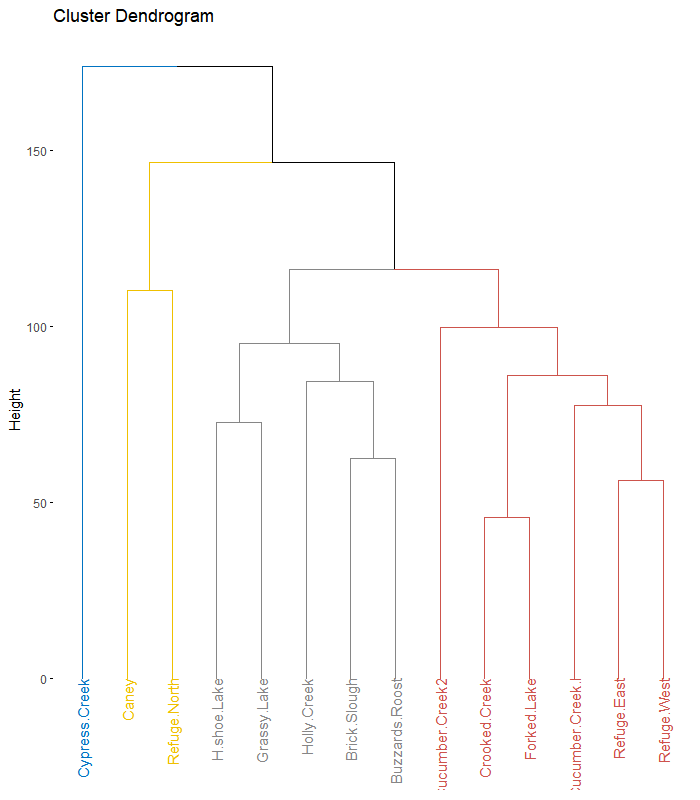
\includegraphics[width = .70\textwidth]{Rplot08.png}
      \end{center}
  \end{figure}

  \textbf{Code:}
  \begin{center}
  \lstinputlisting[basicstyle = \footnotesize]{r5.txt}
  \end{center}

  Comparing the two clustering methods, kmeans and the average linkage euclidean distance agglomerative hierarchical clustering produced the same clusters. This 
  can be seen by reading the print out and noting that the observations are grouped in the same way (had a hard time visualizing this in a systematic way since the methods produced different labels for the clusters).
  

  \begin{footnotesize}
    \begin{verbatim}
      kmeansWoodySpecies <- kmeans(dat_t, centers = 4)
        > kmeansWoodySpecies$cluster
        Cypress.Creek    Crooked.Creek      Forked.Lake Cucumber.Creek.l 
        3                4                4                4 
        Cucumber.Creek2      Refuge.East      Refuge.West            Caney 
        4                4                4                2 
        Refuge.North      H.shoe.Lake     Brick.Slough      Grassy.Lake 
        2                1                1                1 
        Buzzards.Roost      Holly.Creek 
        1                1 
    
    
      cutCompare <- cutree(HclustWoodySpecies, k = 4)
        > cutCompare
        Cypress.Creek    Crooked.Creek      Forked.Lake Cucumber.Creek.l 
        1                2                2                2 
        Cucumber.Creek2      Refuge.East      Refuge.West            Caney 
        2                2                2                3 
        Refuge.North      H.shoe.Lake     Brick.Slough      Grassy.Lake 
        3                4                4                4 
        Buzzards.Roost      Holly.Creek 
        4                4 
    \end{verbatim}
  \end{footnotesize}
  \vspace{.25in}

  \item[e.] Use the cut() function to cut the tree at some level and plot the part of the dendrogram above that cut.\\
  \solution 

  \begin{figure}[H]
    \begin{center}
      \caption{Cut() with 4 Clusters}
    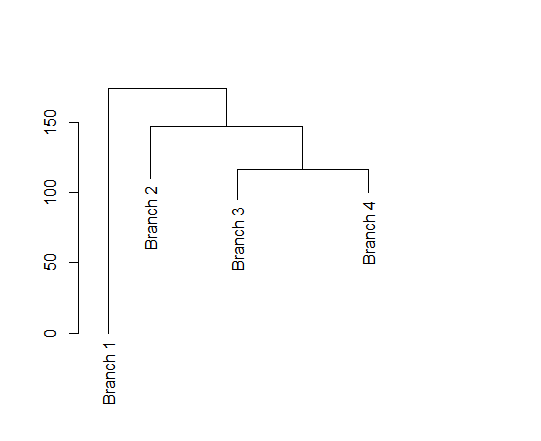
\includegraphics[width = .70\textwidth]{Rplot09.png}
    \end{center}
\end{figure}

  \textbf{Code:}
  \begin{center}
  \lstinputlisting[basicstyle = \footnotesize]{r6.txt}
  \end{center}

\end{enumerate}
  
\end{exercise}
\vspace{.5in}


\begin{exercise}{3} Continue the analysis from the last problem (WoodySpecies data). Here you will look at cophenetic correlation and tanglegrams.\\
  \begin{enumerate}
    \item[a.] What is cophenetic correlation? What is it used for?\\
    \solution  A cophenetic distance, is the distance matrix for a set of data generated from the hierarchical cluster. Cophenetic correlation is what we use 
    to compare the structure of the original distance matrix of the data, and the clustered distance of our data, similar to how a mantel test would be used.
    \vspace{.15in}
    
    
    \item[b.] Using the dendrogram from part (d), problem two, find the correlation between the cophenetic distance matrix and the regular distance matrix.\\
    \solution  \\
    \textbf{Code:}
    \begin{center}
    \lstinputlisting[basicstyle = \footnotesize]{r7.txt}
    \end{center}
    \vspace{.15in}

    \item[c.] You should now compute another hierarchical clustering using a different method from what you used in the 
    last problem and save the dendrogram. Using the tanglegram() function in dendextend package, examine whether this new dendrogram give similar clusters to the 
    dendrogram from the last problem.\\ 
    \solution Computing a new clustering using single linkage, and generating a tanglegram we get the following, 
    \begin{figure}[H]
      \begin{center}
        \caption{Tanglegram: Average Linkage vs. Single Linkage}
      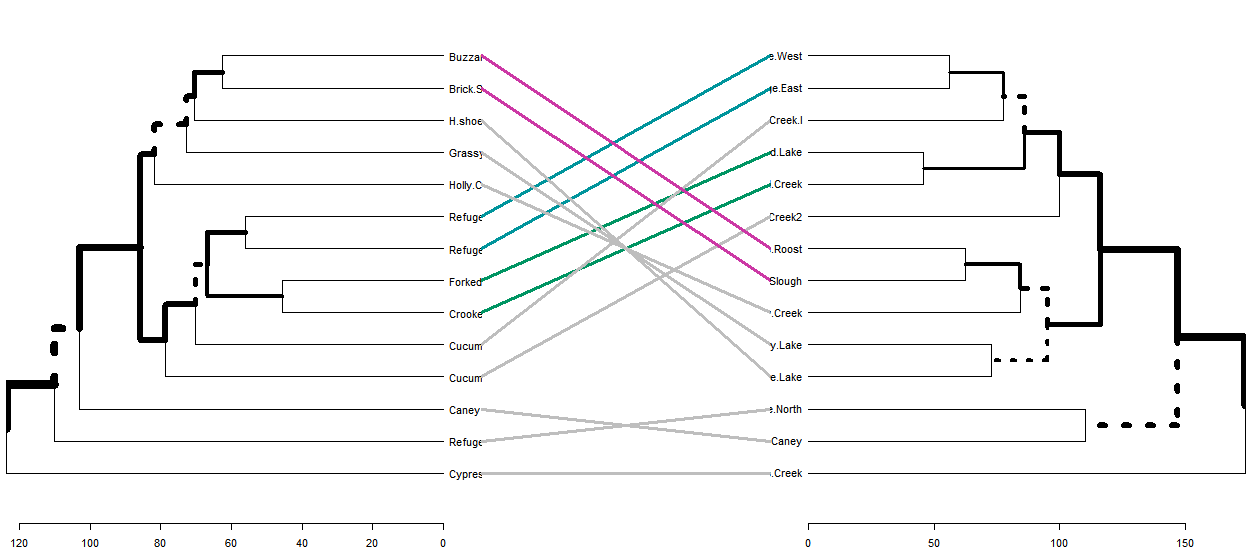
\includegraphics[width = \textwidth]{Rplot10.png}
      \end{center}
  \end{figure}
  \textbf{Code:}
  \begin{center}
  \lstinputlisting[basicstyle = \footnotesize]{r8.txt}
  \end{center}
  From the tanglegram we can see that really the only observations that really separated between the two 
  clustering paradigms where Cucumber.Creek1 and Cucumber.Creek2. Computing the cophenetic correlation we get a value of .97 which makes 
  sense given the tanglegram, shows us generally the same clusters. 
  \end{enumerate}
\end{exercise}
\vspace{.5in}



\begin{exercise}{4} 
  \begin{enumerate}
    \item[a.] What is a divisive hierarchical technique, as opposed to an agglomerative hierarchical technique?\\
    \solution Divisive clustering begins by partitioning the data into one partition, then uses some rule to split the partition into two. This is then repeated 
    until all the data is divided into their own partitions(like decision trees). Agglomerative clustering goes in the other direction by starting with each data in their own partition 
    and using some rule to join partitions together until we form a single partition. 
    \vspace{.15in}
    
    \item[b.] Use code similar to the code below to run DIANA on the Woody Species data.\\
    \begin{footnotesize}
      \begin{verbatim}
      library(cluster)
      res.diana <- diana(distmat, stand = TRUE)
      
      # Plot the dendrogram
      library(factoextra)
      fviz_dend(res.diana, cex = 0.5,
          k = 4, # Cut in four groups
          palette = "jco" # Color palette
          )
      \end{verbatim}
      \end{footnotesize}
      \solution Running the code to generate the plot for the divisive clustering paradigm, 

      \begin{figure}[H]
        \begin{center}
          \caption{Divisive Clustering of WoodySpecies Data.}
        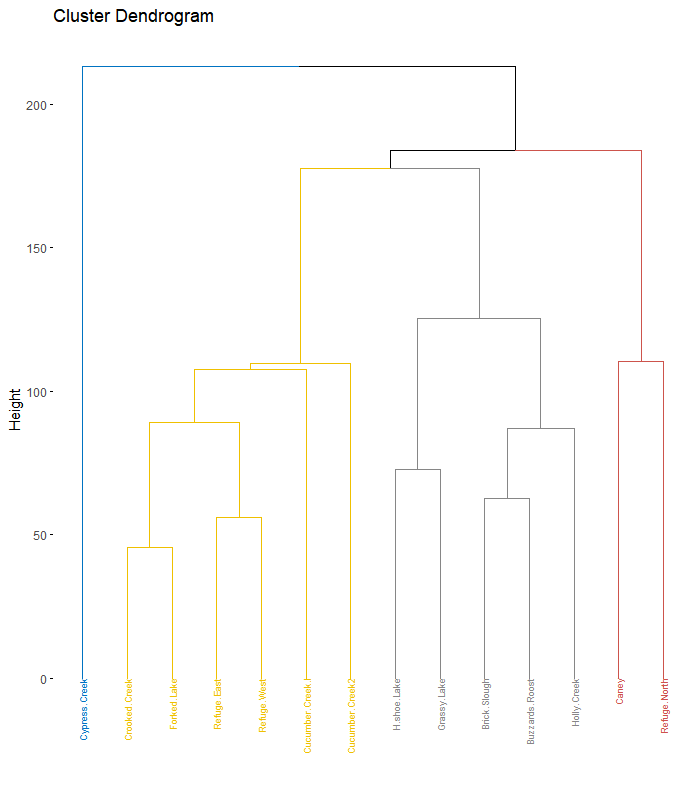
\includegraphics[width = .70\textwidth]{Rplot11.png}
        \end{center}
    \end{figure}

    Generating a tanglegram, and computing the cophenetic correlation to compare the clustering to the average linkage agglomerative clustering we found very similar clustering. 
    \begin{figure}[H]
      \begin{center}
        \caption{Divisive vs Agglomerative Clustering.}
      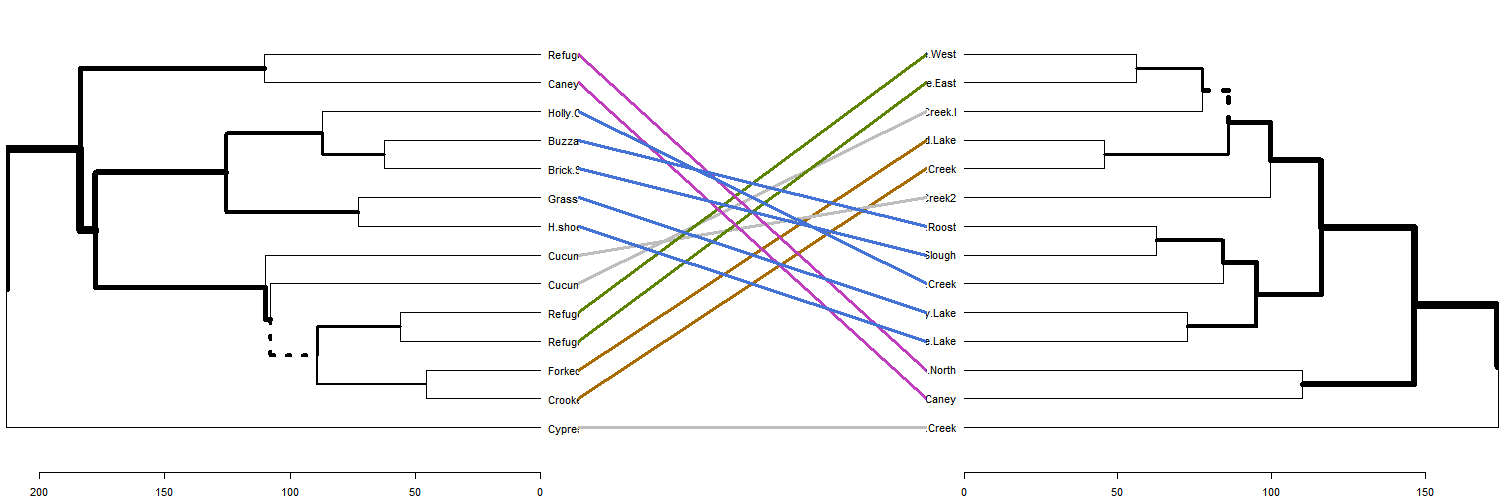
\includegraphics[width = .70\textwidth]{Rplot12.png}
      \end{center}
    \end{figure}

      \textbf{Code:}
      \begin{center}
      \lstinputlisting[basicstyle = \footnotesize]{r9.txt}
      \end{center}
    \end{enumerate}
\end{exercise}

\vspace{.5in}


\begin{exercise}{5} Somewhere, find a dataset that you are interested in that compares multiple sites, countries, etc. Choose your favorite clustering method, 
  then use it to cluster the dataset. How many clusters did you get? why did you pick that number of clusters? Do you think your approach did a good job of clustering?\\
  \solution The data I decided to use comes from Kaggle and it contains information about water quality from 3276 different bodies of water. The goal of the data is to be able to predict the 
  potability of water form metrics like pH, Hardness, Conductivity, Sulfates, and several other predictors. The data also contains labels for each of the observations so we do have 
  a true clustering to compare our methods to. \\
  A kmeans clustering showed that the data contains mainly 2 clusters. The following plots of cumulative and accumulative rsquared show that most of the variance 
  is explained by 2 groups. The two cluster correctly classified 1062 of the 2011 usable observations, which is about as good as randomly assigning labels. 
  \begin{figure}[H]
    \begin{center}
      \caption{Cumulative RSquared from Kmeans Analysis on WaterData}
    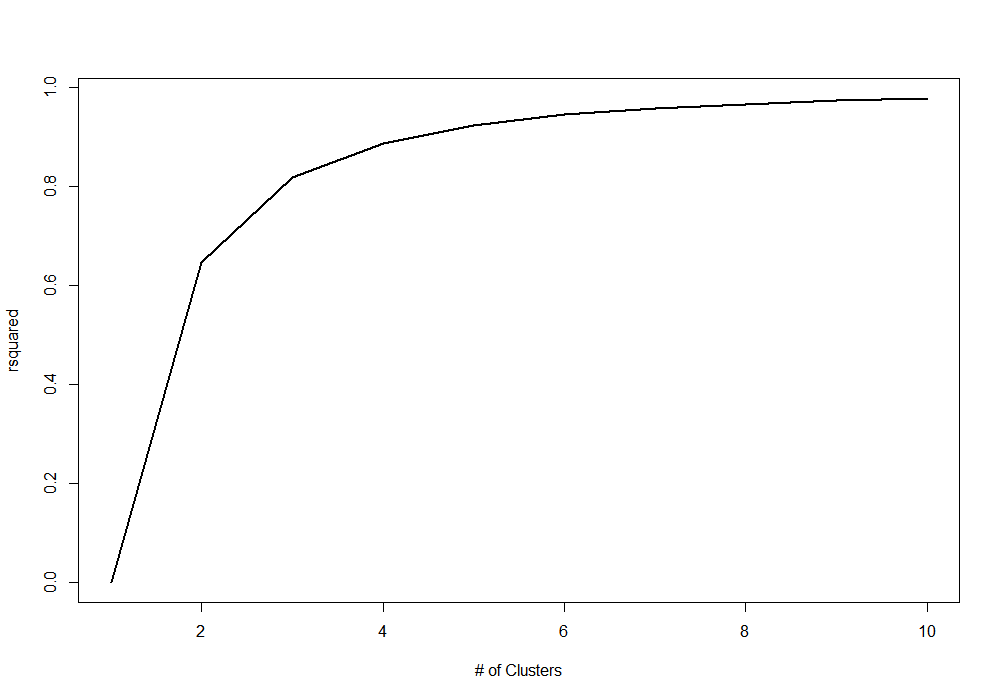
\includegraphics[width = .70\textwidth]{Rplot13.png}
    \end{center}
\end{figure}
\begin{figure}[H]
  \begin{center}
    \caption{Accumulative RSquared from Kmeans Analysis on WaterData}
  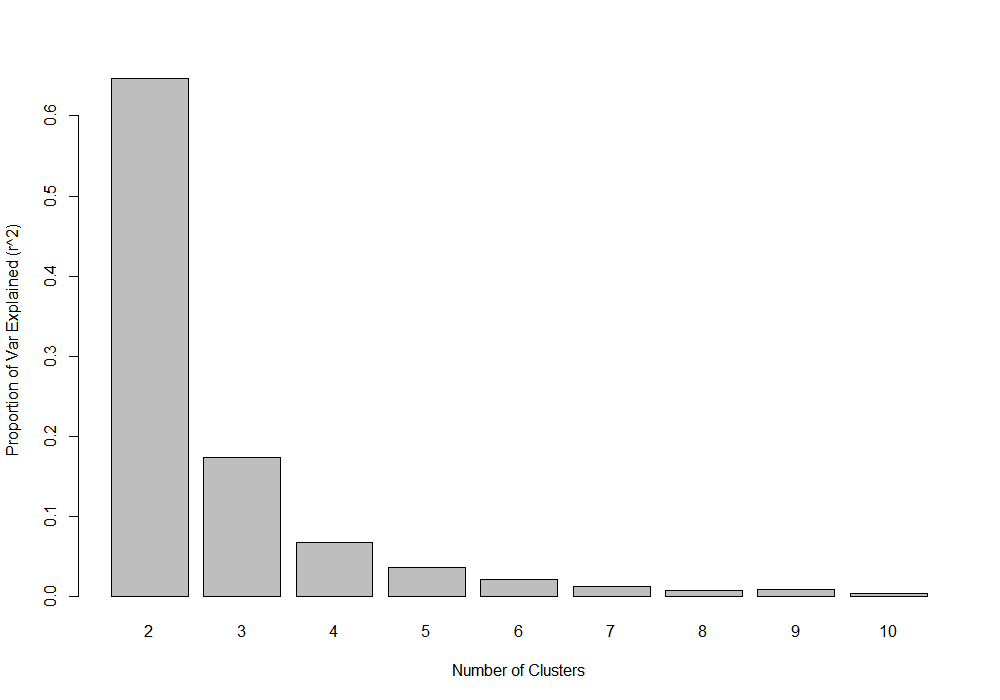
\includegraphics[width = .70\textwidth]{Rplot14.png}
  \end{center}
\end{figure}
\textbf{Code:}
\begin{center}
\lstinputlisting[basicstyle = \footnotesize]{r10.txt}
\end{center}

Things don't get much better when we try the agglomerative hierarchical clustering. Generating the dendrogram for this data is unhelpful (too much data), it shows the same thing as 
the kmeans plots; that two clusters explain a majority of the variance. With the hierarchical clustering we correctly classified 1188 of the 2011 observations, again about as good as random. \\
\textbf{Code:}
\begin{center}
\lstinputlisting[basicstyle = \footnotesize]{r11.txt}
\end{center}
\end{exercise}





\end{document}


















